\section<presentation>[Principes et risques]{Les principes et les risques du filtrage}
  \begin{frame}
    \frametitle{Contexte: un filtre transparent}
    \begin{itemize}
      \item<1-> Filtrer du traffic (web) sans toucher aux connexions TCP.\\
        \only<1>{
          \begin{figure}[h]
            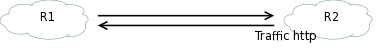
\includegraphics[width=0.8\textwidth]{pictures/filter-before.png}
          \end{figure}
        }
        \only<2->{
          \begin{figure}[h]
            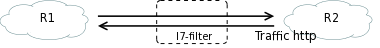
\includegraphics[width=0.8\textwidth]{pictures/filter-after.png}
          \end{figure}
        }
      \item<3-> Cas d'�cole: appliquer des r�gles de QoS restrictives sur les fichiers {\tt .pdf}.
      \item<4-> Hypoth�se: l'un des cot� est neutre (pas de complicit�).
    \end{itemize}
  \end{frame}

  \begin{frame}[t]
    \frametitle{Fonctionnement d'un filtre applicatif}
    Fonctionnement d'un filtre transparent au niveau 7 (OSI):
    \begin{itemize}
      \item<1-> Identification et groupage des packets par session TCP.\\
        \only<1>{\tt\scriptsize
          <tcp src=129.104.201.51 dst=87.98.164.72 sport=4242 dport=80> et \\
          <tcp src=87.98.164.72 dst=129.104.201.51 sport=80 dport=4242>
        }
      \item<2-> Extraction du contenu des buffers egress/ingress.\\
        \only<2>{\tt\scriptsize
          > GET /abcd.pdf HTTP/1.0\\
          > Host: www.blih.org\\
          > \\
          < HTTP/1.1 200 OK\\
          \dots
        }
      \item<3-> D�tection du protocole utilis�.
      \item<4-> Extraction des information (protocol buffer).\\
        \only<4>{\tt\scriptsize
          proto=HTTP, method=GET, url=/abcd.pdf
        }
      \item<5-> Classification finale.\\
        \only<5>{
          Exemple de r�gle: {\tt\scriptsize proto=HTTP method=GET url=.*$\backslash$.pdf}
        }
    \end{itemize}
  \end{frame}

  \begin{frame}
    \frametitle{Attaques et contournement d'un filtre applicatif}
    \begin{itemize}
      \item Contournement via les couches 3/4 OSI.
        \begin{itemize}
          \item Fragmentation des paquets au niveau IP.
          \item R�-arrangement des paquets TCP.
        \end{itemize}
      \item Contournement via l'impl�mentation du protocole
        \begin{itemize}
          \item Contournement par exploitation du protocole
          \item Contournement par leurre du d�tecteur de protocole
          \item Contournement par non-respect du protocole
        \end{itemize}
      \item Attaque \emph{Denial of Service} classique
    \end{itemize}
  \end{frame}

  \begin{frame}
    \frametitle{Contournement par fragmentation des paquets}[t]
    Id�e: utiliser le protocole IP pour casser ``l'atomicit�'' des �changes.
    % FRAG flag, ou paquets � payload r�duit.
  \end{frame}

  \begin{frame}
    \frametitle{Contournement par r�-arrangement des paquets TCP}[t]
    Id�e: changer l'ordre des paquets TCP pour obfusquer le buffer \emph{egress}.
  \end{frame}

  \begin{frame}
    \frametitle{Contournement par exploitation du protocole}[t]
    Id�e: exploiter des fonctionnalit�s obscures (ou pas) du protocole.
    % Keepalive
  \end{frame}

  \begin{frame}
    \frametitle{Contournement par leurre du d�tecteur de protocole}[t]
    Id�e: comettre des erreurs r�cup�rables de nature � leurrer le d�tecteur.
    % Commencer par une erreur en SMTP pour �viter le EHLO.
    % Utiliser des lignes de requete extremement longues, type /././././.....
  \end{frame}

  \begin{frame}
    \frametitle{Contournement par non-respect du protocole}[t]
    Id�e: utiliser des \emph{flavor} peu-connues ou des tol�rances du protocole.
    % Par exemple utiliser "GET <url>\n"
  \end{frame}

  \begin{frame}
    \frametitle{Attaque \emph{Denial of Service} classique}[t]
    Id�e: exploiter les impl�mentations na�ves du protocole.
  \end{frame}
